\section{引力波}

根据微扰轮,二阶引力波的源为一阶标量扰动。由于标量扰动的功率谱在小尺度有一个增强,因而二阶引力波不能简单的被忽略。接下来将给出二阶引力波的运动方程以及功率谱的计算。

\subsection{基本方程}
在共形牛顿规范下,精确到二阶微扰的度规可以写作如下形式
\begin{align}
    ds^2 =
    a^2(\eta)\lbrace-(1+2\Psi)d\eta^2+\lbrack(1-2\Psi)\delta_{ij}+\frac{1}{2}h_{ij}\rbrack
    dx^i dx^j\rbrace,
\end{align}

其中$\Psi$为一阶标量扰动,$h_{ij}$为二阶张量扰动(后文简称张量扰动),并且忽略了一阶张量扰动、矢量扰动和各向异性应力张量扰动部分。

在牛顿规范下,我们可以将张量扰动分解$+$分量和$\times$分量。
\begin{align}
    h_{ij}(\eta,\Vector{x})=\int \frac{d^3\Vector{k}}{{(2\pi)}^{3/2}} e^{i\Vector{k}\cdot\Vector{x}}
    \lbrack
    h^{+}_{\Vector{k}}(\eta)\Unit{e}^{+}_{ij}(\Vector{k}) +
    h^{\times}_{\Vector{k}}(\eta)\Unit{e}^{\times}_{ij}(\Vector{k})
    \rbrack,
\end{align}

其中$\Unit{e}^{+}_{ij}(\Vector{k})$和$\Unit{e}^{\times}_{ij}(\Vector{k})$为极化张量,
且满足正交归一化条件$\sum_{i,j}\Unit{e}^{\alpha}_{ij}(\Vector{k})\Unit{e}^{\beta}_{ij}(-\Vector{k})=\delta^{\alpha\beta}$。
接下来的正文中将忽略极化指标$\alpha$和$\beta$。

结合二阶扰动的爱因斯坦方程,动量空间中的张量扰动满足运动方程
\begin{align}\label{eq:motion_eq_for_hij}
    h^{\dprime}_{\Vector{k}}+2\mathcal{H}h^{\prime}_{\Vector{k}}+k^2h_{\Vector{k}}
    = S(\eta,\Vector{k}),
\end{align}

其中$S(\eta,\Vector{k})$是源项$S_{ij}(\eta,\Vector{k})$的傅立叶变换,
\begin{align}
    S(\eta, \Vector{k}) = -4\Unit{e}^{ij}(\Vector{k})\int
    \frac{d^3\Vector{x}}{{(2\pi)}^{3/2}}
    e^{-i\Vector{k}\cdot\Vector{x}}S_{ij}(\eta,\Vector{k}).
\end{align}

源项的表达式为\citep{ananda2007cosmological,baumann2007gravitational}
\begin{align}
    S_{ij}(\eta,\Vector{k})=
    4\Psi\partial_i\partial_j\Psi + 2\partial_i\Psi\partial_j\Psi-
    \frac{4}{3(1+w)\mathcal{H}^2}\partial_i(\Psi^\prime+\mathcal{H}\Psi)\partial_j(\Psi^\prime+\mathcal{H}\Psi).
\end{align}

利用格林函数法可以给出运动方程 (\ref{eq:motion_eq_for_hij})的解析解
\begin{align}\label{eq:hk_solution}
    h_{\Vector{k}}(\eta)=\frac{1}{a(\eta)}\int^\eta d\tilde{\eta}
    G_k(\eta;\tilde{\eta})\lbrack
    a(\tilde{\eta})S(\tilde{\eta},\Vector{k})\rbrack.
\end{align}

其中$G_k(\eta;\tilde{\eta})$满足如下常微分方程
\begin{align}
    \frac{d^2 G(\eta;\tilde{\eta})}{d\tilde{\eta}^2} + 
    \left(k^2 - \frac{d^2 a}{ad\tilde{\eta}^2}\right)G_k(\eta;\tilde{\eta})
    =
    \delta(\eta-\tilde{\eta}).
\end{align}

为了计算源项$S_{ij}(\eta,\Vector{k})$随时间的演化,需要求解标量扰动的运动方程\citep{mukhanov1992theory,kodama1984cosmological}
\begin{align}
    \Psi^\dprime_{\Vector{k}}(\eta) +
    \frac{6(1+w)}{(1+3w)\eta}\Psi^\prime_{\Vector{k}}(\eta) +
    wk^2\Psi_{\Vector{k}}(\eta) = 0,
\end{align}

其中$w$表示状态方程的参数。标量扰动$\Psi_{\Vector{k}}(\eta)$同时依赖动量$\Vector{k}$和时间$\eta$,分离变量后表示成初值$\psi_{\Vector{k}}$和转移函数$\Psi(k\eta)$的乘积
\begin{align}\label{eq:scalar_pert}
    \Psi_{\Vector{k}}(\eta) \equiv \Psi(k\eta)\psi_{\Vector{k}}.
\end{align}

此时,源项的傅立叶变换可以表示成

\begin{align}\label{eq:source_term}
    S(\eta,\Vector{k}) = \int \frac{d^3 \Vector{p}}{{(2\pi)}^{3/2}}
    \Unit{e}(\Vector{k},\Vector{p}) f(\eta,\Vector{k},\Vector{p})
    \psi_{\Vector{k}}\psi_{\Vector{k-p}},
\end{align}

其中
\begin{align}
    \Unit{e}(\Vector{k,p})=\Unit{e}^{ij}(\Vector{k})p_i p_j,
\end{align}

以及
\begin{equation}
\begin{split}
    f(\eta,\Vector{k,p}) =
    & \frac{8(3w+5)}{3(w+1)}\Psi(|\Vector{p}|\eta)\Psi(|\Vector{k-p}|\eta) + 
    \frac{{4(3w+1)}^2}{3(w+1)}\eta^2\Psi^\prime(|\Vector{p}|\eta)\Psi^\prime(|\Vector{k-p}|\eta)
    \\
    & + \frac{8(3w+1)}{3(w+1)}\eta
    \lbrack
    \Psi^\prime(|\Vector{p}|\eta)\Psi(|\Vector{k-p}|\eta) + 
    \Psi(|\Vector{p}|\eta)\Psi^\prime(|\Vector{k-p}|\eta)
    \rbrack.
\end{split}
\end{equation}

对处于视界内的模式而言,引力波的能量谱的表达式可以通过其功率谱来给出
\begin{equation}\label{eq:gw_energy_spectrum}
    \Omega_{GW}(\eta,k) \equiv \frac{1}{\rho_c}\frac{d\rho_{GW}}{d\ln k}
    = \frac{1}{24}{\left(\frac{k}{\mathcal{H}}\right)}^2
    \overline{\mathcal{P}_h(\eta,k)},
\end{equation}

上划线表示取振荡平均,公式中已经包含了两种极化模式,$\rho_c$为宇宙的临界能量密度。引力波的功率谱$\mathcal{P}_h$定义为
\begin{align}\label{eq:gw_power_spectrum}
    \langle h_{\Vector{k}}(\eta)h_{\Vector{p}}(\eta) \rangle =
    \frac{2\pi^2}{k^3}\delta^3(\Vector{k+p})\mathcal{P}_h(\eta,k).
\end{align}

利用公式 (\ref{eq:hk_solution})和
(\ref{eq:source_term})计算两点关联函数$\langle
h_{\Vector{k}}(\eta)h_{\Vector{p}}(\eta)\rangle$
\begin{equation}
    \langle h_{\Vector{k}}(\eta)h_{\Vector{p}}(\eta)\rangle =
    \int \frac{d^3 q d^3 \tilde{q}}{{(2\pi)}^3}
    \Unit{e}(\Vector{k,
    q})\Unit{e}(\Vector{p,\tilde{q}})I(\eta,\Vector{p,\tilde{q}})
    \langle
    \psi_{\Vector{q}}\psi_{\Vector{k-q}}\psi_{\Vector{\tilde{q}}}\psi_{\Vector{p-\tilde{q}}}
    \rangle,
\end{equation}

其中
\begin{equation}\label{eq:I_integrate}
    I(\eta,\Vector{k,p}) \equiv \int^\eta d\tilde{\eta} 
    \frac{a(\tilde{\eta})}{a(\eta)}
    G_k(\eta;\tilde{\eta})f(\tilde{\eta},\Vector{k,p}).
\end{equation}

我们假设$\psi_{\Vector{k}}$服从高斯分布,根据Wick定理$\psi_{\Vector{k}}$的四点关联函数可以转化为两点关联函数。引入无量纲参数$u\equiv
|\Vector{k-p}|/k$,$v\equiv |\Vector{p}|$和$x\equiv
k\eta$,获得引力波功率谱的最终表达式为\citep{kohri2018semianalytic}
\begin{equation}
    \mathcal{P}_h(\eta,k) = 4\int_0^\infty dv \int_{|1-v|}^{1+v} du 
    \left( \frac{4v^2-{(1+v^2-u^2)}^2}{4uv} \right)
    \mathcal{I}^2(x,u,v)\mathcal{P_R}(ku)\mathcal{P_R}(kv),
\end{equation}

其中
\begin{equation}
    \mathcal{I}(x,u,v) \equiv k^2 I(\eta,\Vector{k, p}).
\end{equation}

对 (4.1)
节讨论的双拐点暴胀模型对应的标量扰动的功率谱而言,其尖峰对应的模式再次进入视界内时,宇宙处于辐射为主的时期,这意味着$w=1/3$。
因此方程 (\ref{eq:scalar_pert})的解和格林函数分别可以化简为
\begin{equation}\label{eq:scalar_pert_simplified}
    \Psi(x) = \frac{9}{x^2}\left(
        \frac{\sin(x/\sqrt{3})}{x/\sqrt{3}}-\cos(x/\sqrt{3})
        \right),
\end{equation}
和
\begin{equation}
    G_k(\eta;\tilde{\eta}) = \frac{\sin(k\eta-k\tilde{\eta})}{k}. 
\end{equation}

峰值对应尺度$10^{13}\text{Mpc}^{-1}$,比基准尺度$k_{\star}=0.05\text{Mpc}^{-1}$大好几个量级。
方程
(\ref{eq:scalar_pert_simplified})说明标量扰动在视界内被抑制,因此诱导引力波的产生期主要集中在对应的模式穿过视界的时候。这个性质使得我们可以使用\citep{kohri2018semianalytic}中提出的方法,当$x\rightarrow
\infty$时,振荡平均的结果为
\begin{equation}
\begin{split}
    & \overline{\mathcal{I}^{2}(x\rightarrow\infty,u,v)} =
    \dfrac{1}{2}{\left(\frac{3}{4u^3v^3x}\right)}^3 {\left(u^2+v^2-3\right)}^2 \\
    &\quad \left\{ {\left[ -4uv+(u^2+v^2-3)\ln\left|\frac{3-{(u+v)}^2}{3-{(u-v)}^2}\right| \right]}^2 +
    {\left[ \pi(u^2+v^2-3)\Theta(u+v-\sqrt{3}) \right]}^2
    \right\},
\end{split}
\end{equation}

其中$\Theta$为Heaviside theta函数。结合方程
(\ref{eq:gw_power_spectrum})和
(\ref{eq:I_integrate})以及辐射为主时期的$\mathcal{H}=1/\eta$,得到最终的表达式
\begin{equation}\label{eq:omega_final}
\begin{split}
    & \Omega_{GW}(\eta,k) = \frac{1}{12}\int_0^\infty dv \int_{|1-v|}^{1+v} du
    {\left(\frac{4v^2-{(1+v^2-u^2)}^2}{4uv}\right)}^2
    \mathcal{P_R}(ku)\mathcal{P_R}(kv) \\
    & \quad {\left(\frac{3}{4u^3v^3}\right)}^2
    {\left(u^2+v^2-3\right)}^2 \\
    &\quad \left\{ {\left[ -4uv+(u^2+v^2-3)\ln\left|\frac{3-{(u+v)}^2}{3-{(u-v)}^2}\right| \right]}^2 +
    {\left[ \pi(u^2+v^2-3)\Theta(u+v-\sqrt{3}) \right]}^2
    \right\}.
\end{split}
\end{equation}

\subsection{数值结果}
在获得$\Omega_{GW}$的数值结果后,我们将其与LISA\citep{amaro2017laser}和太极\citep{guo2018taiji}的灵敏度曲线相比较。
当前时刻与辐射为主时期产生的能量谱之间的关系为
\begin{equation}
    \Omega_{GW,0}=\Omega_{r,0}{\left(\frac{g_{\star,0}}{g_{\star,p}}\right)}^{1/3}\Omega_{GW}, 
\end{equation}

其中$\Omega_{r,0}$为当前辐射能量密度占比,$g_{\star,0}$和$g_{\star,p}$分别为当前时刻和峰值对应的模式穿过视界时的
相对论有效粒子数。当前时刻的频率$f$为
\begin{equation}
    f \approx 0.03\text{Hz}\frac{k}{2\times10^7\text{pc}^{-1}}.
\end{equation}

从图\ref{fig:lisa_taiji}可以看出数值结果位于LISA\citep{amaro2017laser}和太极\citep{guo2018taiji}的期望灵敏度曲线之上。峰值频率的预测值大约为$0.05\text{Hz}$,
落在空间引力波探测器的探测范围内。并且对于在峰值模式$k_p$两侧的模式,可以很好地用$k$的幂函数来描述。当$k\ll
k_p$时,$\Omega_{GW} \propto
k^3$,这与由预加热和相变驱动的随机引力波背景的结果相同。在$k\gg
k_p$的区域内,幂指数为$1.9$,这和其他引力波源的情况不同。

\begin{figure}
    \centering
    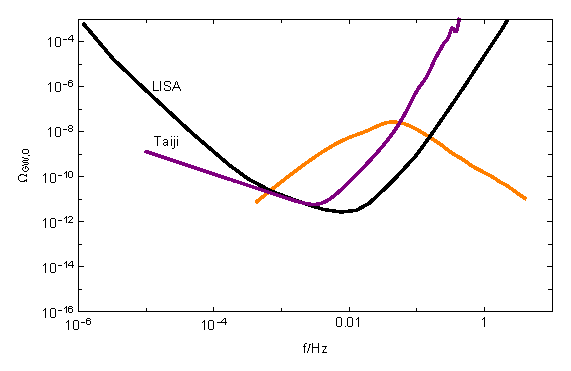
\includegraphics{Img/Lisa2.eps}
    \caption{橙色曲线为双拐点模型预言的诱导引力波的能量谱。黑/红曲线分别为LISA\citep{amaro2017laser}和太极\citep{guo2018taiji}的期望灵敏度曲线。}\label{fig:lisa_taiji}
\end{figure}

\subsection{功率谱为幂指数时的结果}
从图\ref{fig:pert}可以看到原初功率谱在峰值附近可以近似用$k$的幂函数来描述。当$k\ll
k_p$和$k\gg k_p$时,$\mathcal{P_R}(k)\propto
k^{n_1}$和$\mathcal{P_R}(k)\propto k^{n_2}$。此时,$\Omega_{GW}(k)\propto
k^{m_1}$和$\Omega_{GW}(k)\propto
k^{m_2}$。$m_1$和$m_2$是$n_1$和$n_2$的函数。首先看$k\ll
k_p$,$\Omega_{GW}$的主要贡献来自于峰值。因为$v$和$u$反比于$k$,方程
(\ref{eq:omega_final})中对积分的主要贡献来自于区间$1\ll v,u\le
k_p/k$。在这中情况下,,方程 (\ref{eq:omega_final})简化到
\begin{equation}
    \Omega_{GW}(k)\propto k^{2n_1}\int_0^{k_p/k} dv v^{2n_1 - 4}. 
\end{equation}

若$n_1 > 2$,则结果为
\begin{equation}
    \Omega_{GW}(k)\propto k^3.
\end{equation}

再者,考虑第二种情况$k\gg k_p$。若$v\ll 1$或$u\ll
1$,则被积函数能简化为$v^{3-n_2}$。当$n_2 > -4$时,方程
(\ref{eq:omega_final})为
\begin{equation}\label{eq:kp_larger_than_k}
    \Omega_{GW}(k)\propto k^{2n_2}\int_{-\infty}^{+\infty} dv F(v).
\end{equation}

因为
(\ref{eq:kp_larger_than_k})中积分部分与$k$无关,因此$\Omega_{GW}(k)\propto
k^{2n_2}$。对$n_2\le -4$,对积分的主要贡献来自于区间$k_p/k \le v \\
1$或$k_p/k\le u \ll 1$。此时方程 (\ref{eq:omega_final})简化为
\begin{equation}
    \Omega_{GW}(k) \propto k^{2n_2}\int_{k_p/k}^{\epsilon} dv v^{3-n_2},
\end{equation}

其中$\epsilon$满足$k_p/k\ll \epsilon \ll 1$。因此$\Omega_{GW}(k)\propto
k^{n_2-4}$对$n_2 < -4$以及$\Omega_{GW}(k)\propto k^{2n_2-4}$对$n_2=-4$。
